
\chapter{Métodos}

La primera parte de este capítulo presenta la metodología estadística para el análisis de datos provenientes de EMA incluída en el paquete de R y que puede ser empleada interactivamente mediante la aplicación web Shiny. En la segunda y tercera sección, se presenta un flujo de trabajo reproducible para el desarrollo del paquete de R y una descripción de las etapas para la creación de la aplicación web Shiny.


\section{Métodos estadísticos}

\subsection{Modelo AMMI y SREG}
Para el estudio de la IGA y los análisis que de ella se derivan, dos modelos multiplicativos han aumentado su popularidad entre los fitomejoradores como herramientas de análisis gráfico: el modelo de los efectos principales aditivos e interacción multiplicativa (AMMI, siglas en inglés de \emph{Additive Main effects and Multiplicative Interaction}) \citep{Gauch1988, Gauch1992} y el de regresión por sitio (SREG, siglas en inglés de \emph{Site Regression model}) \citep{Corneliusetal1996, CrossaCornelius1997}. Estos modelos se ajustan en dos etapas. Primero, se realiza un ANOVA para obtener estimaciones de los efectos principales aditivos de ambientes y genotipos en AMMI y sólo de los ambientes en SREG. En segundo lugar, los residuos del ANOVA se ordenan en una matriz con genotipos en las filas y ambientes en las columnas y se aplica una DVS, representando los patrones de IGA presentes en los residuos en AMMI y de G e IGA conjuntamente en SREG.\\

Las ecuaciones de los distintos modelos son:

\hspace{0.5cm} AMMI: $y_{ij}= \mu + G_i + A_j + \sum_{k=1}^K \lambda_k \alpha_{ik} \gamma_{jk}$

\hspace{0.5cm} SREG: $y_{ij}= \mu + A_j + \sum_{k=1}^K \lambda_k \alpha_{ik} \gamma_{jk}$ 

donde 
\begin{itemize}
\item $y_{ij}$ es el carácter fenotípico evaluado (rendimiento o cualquier otro carácter de interés) del i-ésimo genotipo en el j-ésimo ambiente,
\item $\mu$ es la media general,
\item  $G_i$ es el efecto del i-ésimo genotipo con $i=1,...,g$,
\item $A_j$ es el efecto del j-ésimo ambiente con $j=1,...,a$,
\item $\sum_{k=1}^K \lambda_k \alpha_{ik} \gamma_{jk}$ es la sumatoria de términos multiplicativos utilizadas para modelar la IGA en AMMI o de G e IGA conjuntamente en SREG. K es el número de términos multiplicativos retenidos en el modelo con $K \leq min(g-1,a-1)$ en AMMI y $K \leq min(g,a-1)$ en SREG; $\lambda_k$ es el k-ésimo valor singular y $\alpha_{ik}$ y $\gamma_{jk}$ son los elementos de los autovectores asociados con el i-ésimo genotipo y el j-ésimo ambiente para el k-ésimo término multiplicativo, respectivamente. En general, los dos primeros términos multiplicativos ($K=2$) son suficientes para explicar los patrones de la IGA en AMMI y de G e IGA en SREG; la variabilidad remanente se interpreta como ruido aleatorio. 
\end{itemize}


El resultado de los dos primeros términos multiplicativos de la DVS se presenta a menudo en un biplot llamado GE (genotipo-ambiente, siglas en inglés de \emph{Genotype-Environment}) para el modelo AMMI \citep{Zobel1988} y GGE (genotipo más genotipo-ambiente, siglas en inglés de \emph{Genotype plus Genotype-Environment}) en SREG \citep{Yanetal2000} y representan una aproximación de dos rangos de los efectos multiplicativos. Dado que para seleccionar cultivares el G e IGA deben considerarse simultáneamente, el modelo SREG resulta superior a AMMI para visualizar patrones en datos provenientes de EMA. Un biplot GGE que explica suficiente variabilidad debida a G e IGA de un conjunto de datos provenientes de EMA permite, entre otras cosas, visualizar tres aspectos importantes: 

\begin{itemize}
\item[(i)] las relaciones entre los genotipos y ambientes representadas por el patrón ``cuál-ganó-donde'' (\emph{which-won-where}), que facilitan la investigación de mega-ambientes \citep{GauchZobel1997}.

\item[(ii)] las interrelaciones entre los ambientes de prueba, que facilitan la identificación de mejores ambientes para la evaluación de cultivares \citep{Cooperetal1997} y de aquellos que son redundantes y pueden descartarse \citep{YanRajcan2002};

\item[(iii)] las interrelaciones entre genotipos en cada mega-ambiente posibilita la comparación entre ellos y la clasificación de los mismos comparándolos con un genotipo ``ideal'' que es aquel con el rendimiento más alto y que es absolutamente estable \citep{Yanetal2001}.  Al compararse el orden de los genotipos en cada mega-ambiente, podría identificarse aquellos con adaptabilidad amplia (el orden del genotipo no varía entre los ambientes), y aquellos con adaptabilidad especifica (sólo muestra buen desempeño en uno o pocos ambientes). Sin embargo, la posibilidad de que algunos genotipos sean seleccionados o no, dependerá de la comparación que se realice con los genotipos controles que se incluyen en los ensayos.
\end{itemize}

Aunque el biplot GGE se usó inicialmente solo para la exploración de los efectos conjuntos de G e IGA, su aplicación se ha extendido a cualquier conjunto de datos que tenga una estructura de doble entrada. En el área de fitomejoramiento en particular, el biplot GGE se ha utilizado para abordar preguntas importantes que es probable que un fitomejorador o investigador plantee. Hasta el momento, ha permitido una visualización holística de la asociación genotipo x carácter, datos de cruces dialélicos, genotipo x marcador, análisis de QTL (siglas en inglés de \emph{Quantitive Trait Loci}) con datos de mapeo, y de interacción planta x patógeno \citep{YanKang2003, Singhetal2020, Hernandezetal2020, Adueral2021}.


En un biplot la puntuación del i-ésimo genotipo en la k-ésima componente principal se muestra como un punto definido por $g_{ik} = \lambda_k^{s} \alpha_{ik}$ y la correspondiente al j-ésimo ambiente en la k-ésima componente por $e_{kj} = \lambda_k^{1-s} \gamma_{jk}$ donde $k=1,2$ para un biplot bidimensional y $s$ es el factor de partición de los valores singulares. Teóricamente, el factor de partición puede tomar cualquier valor entre 0 y 1. Dentro de este rango, la elección de $s$ no altera las relaciones o interacciones relativas entre los genotipos y los ambientes, aunque la apariencia del biplot será diferente. Cuando $s=1$, 
$g_{ik} = \lambda_k \alpha_{ik}$ y $e_{kj} = \gamma_{jk}$, los valores singulares se dividen por completo en los autovectores de los genotipos. En esta escala la unidad de las puntuaciones de los genotipos ($g_{ik}$) es la unidad original del carácter fenotípico evaluado y las puntuaciones ambientales ($e_{kj}$) están normalizadas (es decir no tienen unidad). Cuando $s=0$, $g_{ik} = \alpha_{ik}$ y $e_{kj} = \lambda_k \gamma_{jk}$, los valores singulares se dividen por completo en los autovectores de los ambientes. En esta escala las puntuaciones ambientales están en la unidad original del carácter fenotípico evaluado y las de los genotipos no tienen unidad. Cuando $s=0.5$, $g_{ik} = \lambda_k^{0.5} \alpha_{ik}$ y $e_{kj} = \lambda_k^{0.5} \gamma_{jk}$, la partición es simétrica. En esta escala las puntuaciones de los genotipos y las ambientales tienen la misma unidad que es la raíz cuadrada de la unidad original. El valor de $s=0.5$ es empleado en el biplot GE y el más utilizado en GGE, aunque dependiendo de los intereses de la investigación, se pueden construir numerosas vistas del biplot GGE derivado de SREG. Independientemente del factor de partición en valores singulares utilizado, los biplots GGE revelan el mismo patrón \emph{which-won-where}. Sin embargo, difieren en su precisión al mostrar la interrelación entre ambientes y genotipos. La partición centrada en los genotipos ($s=1$) muestra la interrelación entre genotipos con mayor precisión que cualquier otro método; la partición enfocada en los ambientes ($s=0$) es la más informativa sobre las interrelaciones entre los ambientes; y la simétrica ($s=0.5$) permite visualizar la magnitud relativa tanto de la variación de los genotipos como de los ambientes. 


\subsection{Modelo AMMI robusto}

El modelo AMMI, en su forma estándar, asume que no hay valores atípicos en el conjunto de datos. Sin embargo, la presencia de \emph{outliers} es más una regla que una excepción cuando se consideran datos agronómicos debido a características inherentes de los genotipos que se evalúan, errores de medición o el efecto inesperado de plagas o enfermedades que pueden afectar el rendimiento de algunos genotipos.

\citet{Rodriguesetal2016} proponen una generalización robusta del modelo AMMI, que resulta de ajustar un modelo lineal robusto basado en el estimador M-Huber \citep{Huber1981} y luego utilizar un procedimiento de DVS o de análisis de componentes principales (ACP) robusto. Para la DVS o el ACP los autores consideraron varios métodos, dando lugar a un total de cinco modelos robustos llamados: 

\begin{itemize}
\item R-AMMI: utiliza la DVS robusta propuesta por \citet{Hawkins2002RobustSV} en la cual se reemplaza la norma euclidea por la suma de valores absolutos para calcular una aproximación robusta a la DVS de una matriz rectangular.

\item H-AMMI: se basa en el ACP robusto propuesto por \citet{Hubert2005} que combina las ventajas de un ACP  basado en una matriz de covarianza robusta y uno basado en la búsqueda de proyección.

\item G-AMMI: considera el algoritmo \emph{Grid} robusto propuesto por \citet{Croux2007} que utiliza técnicas de búsqueda de proyección para calcular estimadores del ACP.

\item L-AMMI: utiliza ACP esférico robusto propuesto por \citet{Locantore1999} que consiste en realizar ACP clásico en los datos proyectados en una esfera unitaria.

\item PP-AMMI: considera una técnica de búsqueda de proyección robusta propuesta por \citet{Croux2005} que calcula los autovalores y autovectores secuencialmente sin estimar una matriz de covarianza robusta.
\end{itemize}

El empleo de la versión robusta del modelo AMMI puede ser extremadamente útil debido a que una mala representación de genotipos y ambientes puede resultar en una mala decisión con respecto a qué genotipos seleccionar para un conjunto dado de ambientes \citep{GauchZobel1997, Yanetal2000}. A su vez, la elección de los genotipos incorrectos pueden provocar grandes pérdidas en términos de rendimiento. Los biplots obtenidos de los modelos robustos mantienen las características e interpretación estándar del modelo AMMI clásico \citep{Rodriguesetal2016}.


\subsection{Métodos de imputación}

Una limitación importante que presentan los modelos multiplicativos descriptos previamente es que requieren que el carácter fenotípico bajo estudio se encuentre registrado para todas las combinaciones entre genotipos y ambientes, es decir no admiten valores perdidos. Aunque los EMA están diseñados para que todos los genotipos se evalúen en todos los ambientes, la presencia de valores faltantes es muy común debido a errores de medición o pérdidas de plantas por animales, inundaciones o problemas durante la cosecha, además de la dinámica propia de las evaluaciones en las que se incorporan o descartan genotipos debido a su mal desempeño \citep{HillRosenberg1985}.

Para superar el problema de los datos incompletos, existen diversas soluciones: (i) extraer el subconjunto completo de datos eliminando aquellos genotipos o ambientes con valores faltantes, generando una gran pérdida de información; (ii) completar las celdas incompletas utilizando la media ambiental, lo cual no es una buena estrategia, especialmente cuando la cantidad de valores perdidos es grande; (iii) considerar un método más complejo que permita la falta de datos; y (iv) completar las celdas faltantes con valores estimados utilizando métodos de imputación \citep{GauchZobel1990, Troyanskayaetal2001,Alarconetal2010, Paderewski2013, Alarconetal2014, JosseHusson2016, Alarconetal2020}. Dado que las dos primeras opciones no resultan apropiadas y la tercera complejiza mucho el análisis, en el paquete se incluyen metodologías de imputación para poder ajustar el modelo AMMI o SREG, aún en presencia de valores perdidos, entre las cuales se encuentran: 

\begin{itemize}
\item EM-AMMI: \citet{GauchZobel1990} desarrollaron un procedimiento iterativo que utiliza el algoritmo de maximización de la esperanza (EM, siglas en inglés de \emph{Expectation Maximization}) incorporando el modelo AMMI. Para llevar a cabo este procedimiento, en primer lugar los parámetros aditivos del modelo AMMI se establecen mediante la media general, la de los genotipos y de los ambientes obtenidas a partir de los datos observados. Los residuos de las celdas observadas se calculan como la media de dicha celda menos la media del genotipo menos la media del ambiente más la media general. Los K parámetros multiplicativos del modelo se obtienen al aplicar la DVS sobre la matriz de residuos, y los valores faltantes se completan con las estimaciones de AMMI. En iteraciones posteriores, el procedimiento habitual de AMMI se aplica a la matriz completa y los valores faltantes se actualizan mediante las estimaciones de AMMI correspondientes. Las iteraciones se detienen cuando el cambio entre los valores imputados para las celdas faltantes de dos pasos sucesivos sea pequeño, por ejemplo 0.01. El código de R de esta metodología fue implementado por \citet{Paderewski2013}.
\end{itemize}

\begin{itemize}
\item EM-SVD: \citet{Troyanskayaetal2001} propusieron un método de imputación que combina el algoritmo EM con la DVS. Este método reemplaza los valores faltantes de una matriz inicialmente por valores arbitrarios para obtener una matriz completa, y luego se calcula iterativamente la DVS de esta matriz. Al final del proceso, cuando las iteraciones alcanzan la estabilidad, se obtiene una matriz que contiene las imputaciones de los valores faltantes.
\end{itemize}

\begin{itemize}
\item EM-PCA: \citet{JosseHusson2016} propusieron imputar los valores faltantes de un conjunto de datos utilizando el algoritmo ACP iterativo. Este procedimiento consiste primero en imputar valores perdidos con valores iniciales como la media de la variable. El segundo paso es realizar un ACP en el conjunto de datos completo. Luego, imputa los valores faltantes con las fórmulas de reconstrucción de orden k (la matriz ajustada calculada con una cantidad de componentes ``k'' para los \emph{scores} y cargas). Estos pasos de estimación de los parámetros vía ACP e imputación de los valores faltantes usando la matriz ajustada se iteran hasta la convergencia. 
\end{itemize}

\begin{itemize}
\item GabrielEigen fue propuesto por \citet{Alarconetal2010} y luego fue extendido a una versión ponderada llamada WGabriel \citep{Alarconetal2014}. El primero combina una regresión y aproximación de rango inferior utilizando la DVS. Este método reemplaza inicialmente las celdas faltantes por valores arbitrarios. Posteriormente las imputaciones se actualizan a través de un esquema iterativo que define una partición de la matriz para cada valor faltante y utiliza una regresión lineal de columnas (o filas) para obtener la nueva imputación.  En esta regresión se aproxima la matriz de diseño por una matriz de menor rango utilizando la DVS. WGabriel es una modificación de GabrielEigen que usa pesos elegidos por validación cruzada para imputar los datos.
\end{itemize}

\section{Creación de un paquete de R}

Un paquete de R es un conjunto de funciones programadas en este lenguaje que comparten fines específicos y se distribuyen con un protocolo estandarizado, garantizando su correcto funcionamiento. Para la creación de un paquete se deben seguir ciertas convenciones referidas a la creación y almacenaje de carpetas y archivo con código de programación, documentación e instrucciones de sistema. La gestión de todos estos documentos puede ser manual, pero existen paquetes de R que asisten en la tarea del desarrollo de nuevos paquetes automatizando ciertas fases del proceso. En este trabajo se usaron los paquetes: \emph{devtools} \citep{Wickhametal2021}, \emph{usethis} \citep{WickhamBryan2021}, \emph{roxygen2} \citep{Wickhametal2020}, \emph{testthat} \citep{Wickham2011} y \emph{available} \citep{Ganzetal2019}. 

Una vez finalizada esta etapa, dichas carpetas y archivos se compilan y comprimen para su distribución. Si esto se realiza con Windows como sistema operativo, se debe descargar e instalar el software Rtools disponible en CRAN. 

Todo este proceso se realizó utilizando Git y GitHub. Git es un sistema de control de versiones, una herramienta que toma inicialmente una versión de un documento y luego registra los cambios que sufre el mismo a lo largo del tiempo. Esto facilita el trabajo colaborativo entre distintas personas ya que si más de una persona trabaja en el mismo documento, el sistema de control de versiones las puede integrar en una nueva. Git es más útil cuando se combina con GitHub. Este último es el servicio de \emph{hosting} que se utiliza para que el proyecto tenga una presencia en la web permitiéndole a otras personas explorar los archivos, su historia, sincronizarse con la versión actual, proponer y realizar cambios, etc. Git y GitHub en conjunto forman el entorno más popular para los desarrolladores de paquetes de R ya que permite a cualquier persona descargar e instalar un paquete e incluso realizar aportes, detectar errores, incluir sugerencias, etc.


A continuación se detallan los distintos pasos que componen la creación de un paquete en R bajo un enfoque de trabajo reproducible, lo cual significa que los mismos pueden usarse de ejemplo para el desarrollo de nuevos paquetes o para imitar la creación del paquete \emph{geneticae} que es objeto de desarrollo de este trabajo. 

\subsection{\emph{geneticae}}

En primer lugar se debe elegir el nombre del paquete cumpliendo con ciertas reglas: solo puede contener letras, números o puntos; debe tener al menos dos caracteres y empezar con una letra y no terminar con un punto. Se debe chequear si el nombre elegido está disponible en los repositorios  CRAN, Bioconductor y GitHub. Para ello, se utiliza la función \textcolor{fandango}{available()} del paquete \emph{available}, que además indicará si el nombre elegido tiene algún significado especial que podemos desconocer (revisa las webs de \emph{Wikipedia}, \emph{Wiktionary} y \emph{Urban Dictionary}). El nombre elegido en este caso fue ``geneticae''  (Figura \ref{fig:fig31}). 

\begin{figure}[h]
\begin{center}
	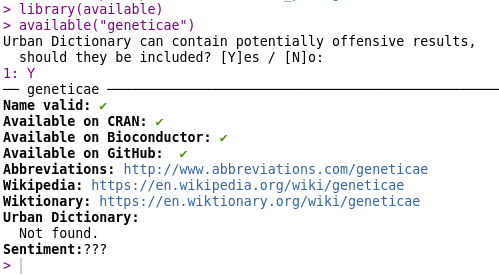
\includegraphics[width=0.50\textwidth]{./Graficos/available.png}	
\end{center}
	\caption{Chequeo de disponibilidad del nombre \emph{geneticae} elegido para el paquete en desarrollo mediante la función \textcolor{fandango}{available()} del paquete \emph{available}.}
\label{fig:fig31}
\end{figure}


\subsection{Estructura general del paquete}

Un paquete de R se construye creando y guardando diversos archivos y carpetas en un directorio cuyo nombre es igual al elegido en el paso anterior. Algunos elementos son de presencia obligatoria, entre ellos:

\begin{itemize}
\item Archivo DESCRIPTION: archivo de texto que describe el contenido del paquete, quiénes son sus desarrolladores, establece cómo se va a relacionar con otros, el tipo de licencia con el que se distribuye, los requisitos de sistema, etc.
\item Carpeta R: contiene el o los archivos de código (\emph{scripts}) de R con las funciones del paquete.
\item Carpeta man: incluye archivos con la documentación del paquete, funciones y \emph{datasets}.
\item README: archivo de texto que brinda información sobre el proyecto.
\item Archivo NAMESPACE: declara las funciones del paquete que se ponen a disposición de los usuarios y lista las funciones de otros paquetes de las cuales hace uso. 
\end{itemize}

Existen otros elementos cuya inclusión es opcional, por ejemplo:

\begin{itemize}
\item Carpeta data: contiene objetos de R con conjuntos de datos.
\item Carpeta vignettes: contiene los tutoriales que muestran ejemplos de uso del paquete, generalmente escritos en Rmarkdown, un formato de escritura que
facilita la presentación de texto entrelazado con código y resultados.
\item Carpeta tests: incluye código que permiten someter al paquete a diversos controles.
\end{itemize}

Si bien estas carpetas y archivos pueden crearse en forma manual, es conveniente utilizar la función \textcolor{fandango}{create\_package()} del paquete \emph{usethis} que se encarga de generar automáticamente un directorio con todas las componentes requeridas para el desarrollo del paquete que sirve de plantilla para facilitar la parte inicial de este proceso (Figura \ref{fig:fig32}). 

\begin{figure}[h]
	\begin{center}
		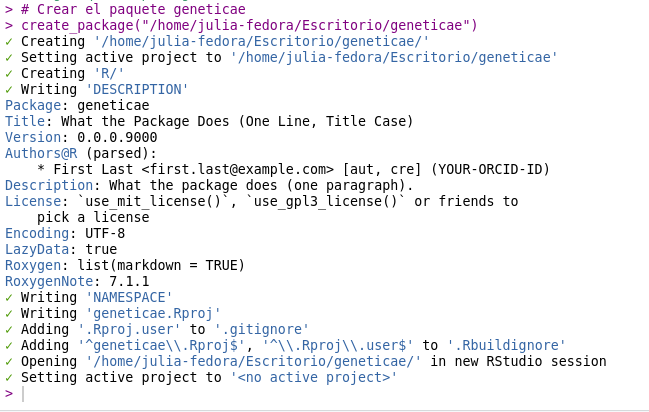
\includegraphics[width=0.60\textwidth]{./Graficos/creacion2.png}	
	\end{center}
	\caption{Creación del paquete \emph{geneticae} mediante la función \textcolor{fandango}{create\_package()} del paquete \emph{usethis}.}
	\label{fig:fig32}
\end{figure}


\subsection{Archivo DESCRIPTION}
\label{subsec:description}
El archivo DESCRIPTION provee toda la metadata sobre el paquete presentada a través de campos, algunos de los cuales tienen que estar de forma obligatoria y otros son opcionales. Los campos obligatorios son: 

\begin{itemize}
\item Package: nombre del paquete.
\item Title: título del paquete (hasta 65 caracteres).
\item Version: número de la versión actual del paquete, en este caso 0.1.9000.
\item Author, Maintainer o Authors@R: autores, contribuyentes y personas a cargo del mantenimiento del paquete.
\item Description: descripción del paquete.
\item License: nombre de la licencia bajo la cual se distribuye el paquete. Si se pretende que cualquiera lo puede usar, entonces se debe recurrir a los tipos más comunes de licencia para código abierto: CC0, MIT o GPL. 
\end{itemize}

Entre los campos opcionales los más improtantes son:
\begin{itemize}
\item Imports: en el caso de que el código desarrollado haga uso de funciones pertenecientes a otros paquetes, los mismos deben ser listados en este campo.
\item Suggests: listado de paquetes que no son imprescindibles para el uso del nuevo paquete, pero que pueden ser útiles como herramientas secundarias para el mismo (por ejemplo, para seguir los tutoriales).
\item Depends: mínima versión de R con la cual el paquete es compatible.
\item URL: dirección de la página web del paquete.
\item BugReports: dirección donde los usuarios pueden enviar avisos sobre los problemas que encuentren al utilizar el paquete.
\end{itemize}

El archivo DESCRIPTION del paquete \emph{geneticae} se muestra en la Figura \ref{fig:fig33}.

\begin{figure}[p]
	\begin{center}
		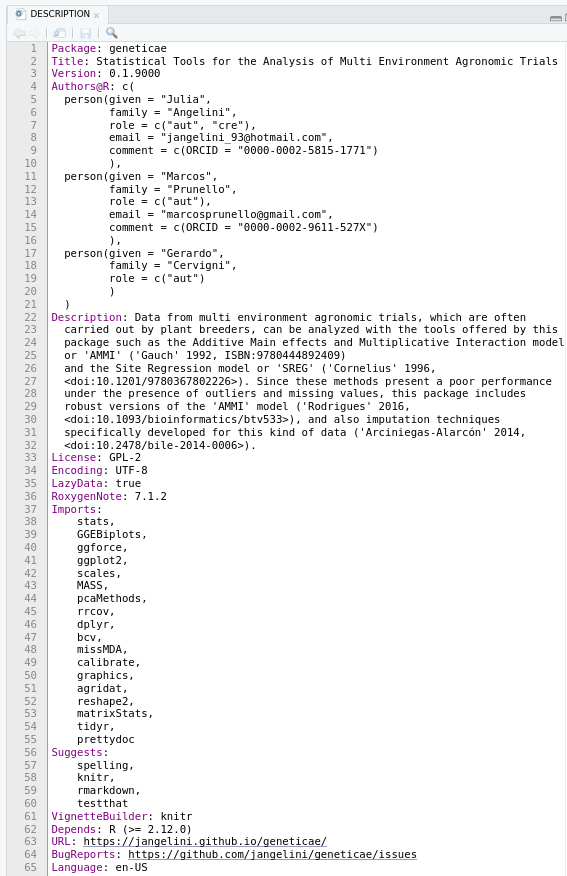
\includegraphics[width=0.50\textwidth]{./Graficos/DESCRIPTION2.png}	
	\end{center}
	\caption{Archivo DESCRIPTION de \emph{geneticae}.}
	\label{fig:fig33}
\end{figure}


\subsection{Archivos de código}

Una vez creada la estructura del paquete y el archivo DESCRIPTION se deben programar las funciones que el mismo contendrá. Estas deben ser guardadas en \emph{scripts} con extensión .R, en el subdirectorio R/. Los \emph{scripts} pueden contener código para una o más funciones y ser guardadas con cualquier nombre, aunque es recomendable que el mismo esté relacionado con su contenido. La Figura \ref{fig:fig34} muestra un fragmento de la función \textcolor{fandango}{GGEmodel()} del paquete \emph{geneticae}.

\begin{figure}[p]
	\begin{center}
		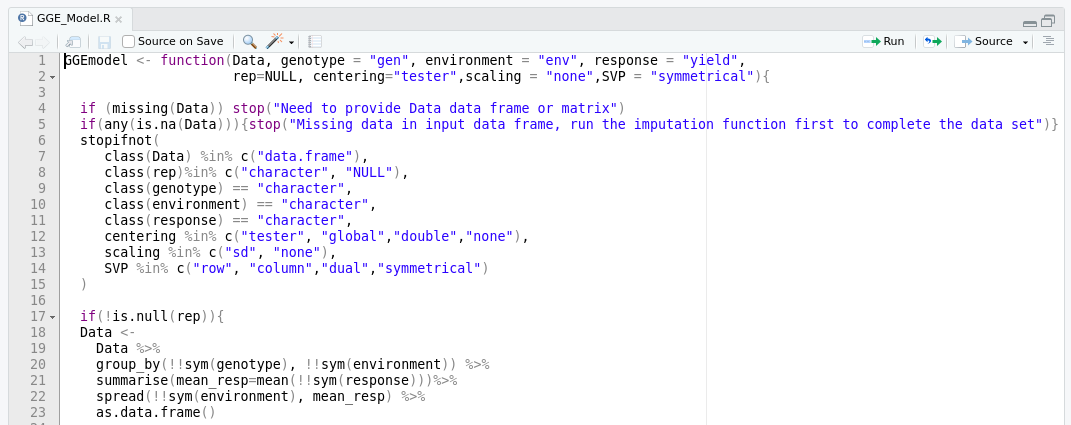
\includegraphics[width=0.55\textwidth]{./Graficos/GGEMODELFUNCTION.png}	
	\end{center}
	\caption{Fragmento de la función \textcolor{fandango}{GGEmodel()} del paquete \emph{geneticae}.}
	\label{fig:fig34}
\end{figure}


A medida que se desarrolla el paquete se van generando relaciones complejas entre las funciones programadas. Algunas de ellas son de uso interno (son invocadas por otras funciones del paquete para cumplir con alguna tarea específica) y otras son diseñadas para que estén disponibles para los usuarios (es decir, se ``exportan"). Además algunas funciones invocan a otras pertenecientes a paquetes escritos por terceros. Esto hace necesario realizar pruebas del funcionamiento del código  producido durante todo el proceso de desarrollo para garantizar que realice lo que realmente se desea y para corregir errores en la programación (depuración o \emph{debugging}). Para simular el proceso de construcción, instalación y carga del paquete durante su desarrollo se utiliza la función 
\textcolor{fandango}{load\_all()} de \emph{devtools} que permite acceder a las funciones del paquete para su evaluación.


\subsection{Documentación}

Uno de los aspectos más importantes de la creación de un paquete es la documentación donde se describe cómo se usa cada función y para qué sirven los argumentos, se aclara qué tipo de resultado devuelve, se proveen ejemplos para el uso, etc. El paquete \emph{roxygen2} provee pautas para incluir todo esto escribiendo comentarios con un formato especial antes de la definición de la función en el mismo archivo de código. 

El flujo de trabajo para crear la documentación con el paquete \emph{roxygen2} es el siguiente:

\begin{enumerate}

\item Agregar comentarios a los archivos .R. Estos deben comenzar con \#', para distinguirlo de los comentarios regulares y preceden a cada función. La primera línea es el título y el párrafo que le sigue es su descripción. Para el resto de los campos de la documentación, se utilizan etiquetas listadas línea tras línea que comienzan con @, siendo las más importantes a incluir:

\begin{itemize}
\item @param: detalla para qué sirve cada parámetro de la función, qué tipo de objeto es y qué valor toma por defecto (opcional).
\item @return: explica qué objeto devuelve la función.
\item @details: agrega cualquier aclaración que se considere necesaria.
\item @examples: incluye ejemplos de uso de la función.
\item @export: indica que la función tiene que estar disponible cuando alguien cargue el paquete con \textcolor{fandango}{library()}.
\item @references: inserta referencias bibliogŕaficas.
\end{itemize}

\item Ejecutar \textcolor{fandango}{document()} del paquete \emph{devtools} para convertir los comentarios escritos en formato roxygen en los archivos que compondrán el manual de ayuda y que deben ir guardados en la carpeta man. Además, esto se encarga de generar el archivo NAMESPACE, que tiene como objetivo declarar cuáles son las funciones del nuevo paquete que son para exportar, así como también listar todas las fuciones importadas de otros paquetes.

\end{enumerate}

La Figura \ref{fig:fig35} muestra un fragmento de los comentarios roxygen de la función \textcolor{fandango}{GGEmodel()} del paquete \emph{geneticae}.

\begin{figure}[h]
	\begin{center}
		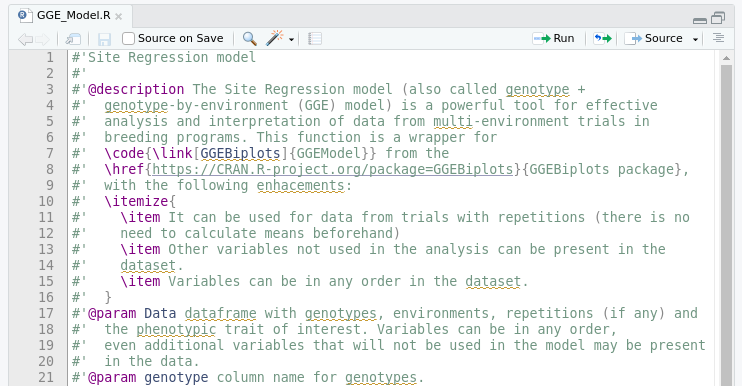
\includegraphics[width=11cm]{./Graficos/COMENTARIOSROXYGEN.png}	
	\end{center}
	\caption{Fragmento de los comentarios roxygen de la función \textcolor{fandango}{GGEmodel()} del paquete \emph{geneticae}.}
	\label{fig:fig35}
\end{figure}


\subsection{Uso de funciones de otros paquetes}
Cuando el código desarrollado invoca a funciones de otros paquetes, los mismos deben ser listados en el campo Imports del archivo DESCRIPTION como se mencionó en la sección \ref{subsec:description}. Esto puede hacerse de manera manual o mediante la función \textcolor{fandango}{use\_package()} del paquete \emph{devtools} indicando el nombre del paquete.

En el código se debe hacer uso de tales funciones anteponiendolo a su nombre el del paquete y el operador ``::". Por ejemplo, \textcolor{fandango}{dplyr::group\_by()} invoca la función \textcolor{fandango}{group\_by()} del paquete \emph{dplyr}. En el caso de que alguna función se aplicara con mucha frecuencia, se puede prescindir del comando anterior si se agrega el nombre de la función y el paquete de procedencia en la etiqueta \textcolor{fandango}{@importFrom} en los comentarios roxygen. Para el ejemplo anterior se debería indicar \textcolor{fandango}{@importFrom dplyr group\_by}. Esto permite mencionar a la función en el código sin el operador ``::".

Si se utilizan repetidamente muchas funciones de otro paquete, es posible importarlas todas indicando el nombre del mismo en la etiqueta \textcolor{fandango}{@import} en los comentarios roxygen. Sin embargo, esta es la solución menos recomendada porque hace que el código sea más difícil de leer y aumenta la posibilidad de que entren en conflicto nombres de funciones pertenecientes a diversos paquetes.

\subsection{Testeos}

Probar el código desarrollado, somentiéndolo a casos particulares y a distintos ejemplos, es fundamental en la creación de paquetes ya que permite detectar y corregir errores y asegurarse que el código haga lo que realmente se desea.

Como se mencionó anteriormente, esto puede hacerse de manera dinámica e interactiva durante el desarrollo al instalar y cargar el paquete en gestación con \textcolor{fandango}{load\_all()}. Sin embargo, si siempre se realizan los mismos controles es posible automatizar este proceso. Para ello, se generan unidades de testeo que ponen a prueba el código corriendo parte del mismo bajo distintas circunstancias y comparando el resultado obtenido con el esperado por el desarrollador.  La función \textcolor{fandango}{use\_test()} del paquete \emph{testthat}, que agrega ``testthat'' al campo Suggest del archivo DESCRIPTION, crea un directorio test/testthat para ubicar los códigos con los testeos y un archivo testthat.R que se encarga de la ejecución de los mismos. Una vez escritos estos archivos que establecen cuales son los controles a realizar automáticamente, se pueden evaluar los resultados con la función \textcolor{fandango}{test()} del paquete \emph{devtools}. Ante cada error encontrado, se debe corregir el código y repetir este proceso hasta que todas las unidades de testeo pasen la prueba. En la Figura \ref{fig:fig36} se muestra el resultado de evaluar las unidades de testeo creadas para el paquete \emph{geneticae}.

\begin{figure}[H]
	\begin{center}
		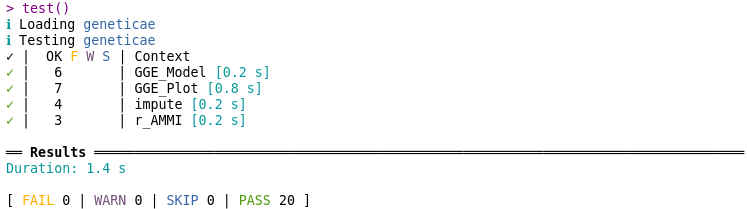
\includegraphics[width=11cm]{./Graficos/Test.png}	
	\end{center}
	\caption{Resultado de correr la función \textcolor{fandango}{test()} del paquete \emph{devtools} en \emph{geneticae}.}
	\label{fig:fig36}
\end{figure}

Una medida de la calidad de un paquete está dada por el porcentaje de código que es evaluado durante los testeos. Esta se puede obtener mediante la función \textcolor{fandango}{test\_coverage()} del paquete \emph{covr} \citep{Hester2020}. El paquete \emph{geneticae} tiene un porcentaje total de cobertura de los test igual a 24.75\% (Figura \ref{fig:fig37}).

\begin{figure}[H]
	\begin{center}
		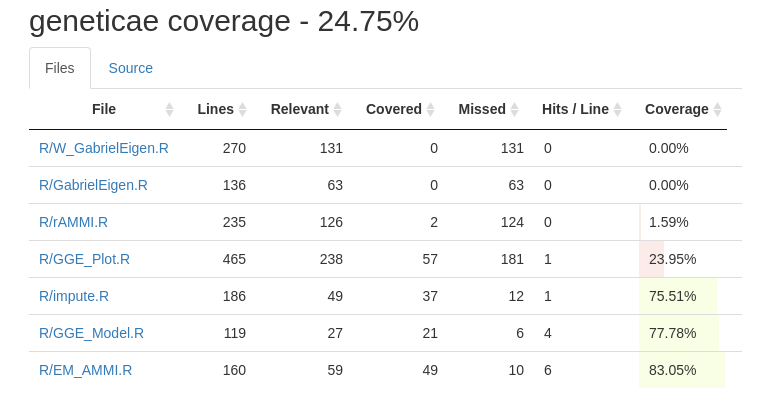
\includegraphics[width=10cm]{./Graficos/Cobertura.png}	
	\end{center}
	\caption{Porcentaje del código de \emph{geneticae} que es evaluado durante los testeos obtenido mediante la función \textcolor{fandango}{test\_coverage()} del paquete \emph{covr}.}
	\label{fig:fig37}
\end{figure}


\subsection{\emph{Datasets}}

A menudo es útil incluir conjuntos de datos en un paquete a fin de proporcionar ejemplos de uso de las funciones incluidas. Los \emph{datasets} que se deseen añadir a un paquete deben ser guardados como archivos .RData en el directorio data/. La función \textcolor{fandango}{use\_data()} del paquete \emph{usethis} puede ser empleada para automatizar este proceso.

Los objetos de la carpeta data siempre se exportan, por lo cual se debe agregar documentación para los mismos. Esto se puede incluir en cualquier archivo de código .R dentro del directorio R/. 


\subsection{Archivo README}

Un README es un archivo de texto plano que se utiliza para documentar o brindar información sobre alguna pieza de software o proyecto. Si un directorio contiene un archivo README, se espera que el usuario lo lea antes de explorar el resto del contenido. En el contexto de creación de paquetes de R, el README se suele escribir en RMarkdown y describe brevemente por qué y para qué alguien podría usar el paquete, junto con menciones para su instalación y un ejemplo introductorio. Además, este archivo se muestra en la página del paquete cuando este es publicado en plataformas como GitHub. 

Para generar el README se utiliza la función \textcolor{fandango}{use\_readme\_rmd()} del paquete \emph{usethis} que crea un archivo de Rmarkdown con una plantilla donde se completa su contenido. 

En el archivo README se suelen incluir insignias (``bagdes") y el logo del paquete. Algunas funciones del paquete \emph{usethis} permiten agregar las insignias al README. Por otro lado, muchos de los paquetes de R disponen de un logo con forma hexagonal conocido como hexSticker. Esto permite darle identidad al paquete. El logo se puede crear con ayuda del paquete \emph{HexSticker} y ser añadido al README con la función \textcolor{fandango}{use\_logo()}. La Figura \ref{fig:fig38} presenta un fragmento del archivo README mostrado en el respositorio GitHub del paquete \emph{geneticae}.

\begin{figure}[h]
	\begin{center}
		
\includegraphics[width=11cm]{./Graficos/README2.png}	
	\end{center}
	\caption{Fragmento del archivo README mostrado en el respositorio GitHub del paquete \emph{geneticae}.}
	\label{fig:fig38}
\end{figure}


\subsection{Archivo NEWS}

El archivo NEWS se encarga de contar los cambios presentes en cada versión nueva del paquete que se publica. Mientras que el README apunta a ser leído por nuevos usuarios, el archivo NEWS es para aquellos que ya usan el paquete.

Se sugiere usar RMarkdown para escribir este archivo y colocar un título principal para cada versión, seguido por títulos secundarios que describen lo realizado (cambios principales, errores arreglados, etc.). Si se trata de cambios impulsados por otras personas, por ejemplo, a través de sugerencias hechas en GitHub, se los menciona para darles mérito. Una buena práctica es ir escribiendo este archivo cada vez que se realiza algo nuevo en el paquete. La función que permite crear este archivo automáticamente es \textcolor{fandango}{use\_news\_md()} del paquete \emph{usethis}. 

La Figura \ref{fig:fig39} presenta el contenido del archivo NEWS del paquete \emph{geneticae}.

\begin{figure}[h]
	\begin{center}
		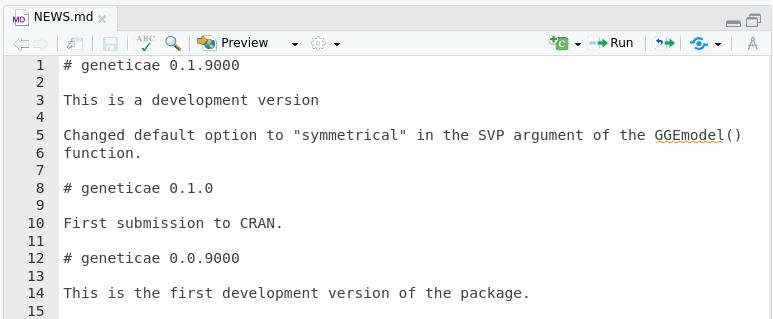
\includegraphics[width=11cm]{./Graficos/News.png}	
	\end{center}
	\caption{Archivo NEWS de \emph{geneticae}.}
	\label{fig:fig39}
\end{figure}


\subsection{Viñetas}

Una viñeta es un tipo especial de documentación que puede agregarse al paquete para dar más detalles y ejemplos sobre el uso del mismo. En ella se brinda una descripción del problema que el paquete está diseñado para resolver y se muestra al lector cómo resolverlo. Se diferencian de las páginas de ayuda en que su adición es opcional y no sigue una estructura fija, dándole la libertad al autor de enseñar de la forma que más le guste cómo usar su paquete. 


Muchos de los paquetes existentes tienen viñetas a las que se puede acceder utilizando la función \textcolor{fandango}{browseVignettes(``nombre del paquete")} si el mismo se encuentra instalado o consultando en su página de CRAN. Por ejemplo para el paquete \emph{geneticae}: \url{https://cran.r-project.org/web/packages/geneticae/vignettes/a-tutorial.html}.

Generalmente, las viñetas son generadas en RMarkdown. Para crear viñetas se emplea la función \textcolor{fandango}{use\_vignette(``nombre del paquete'')} del paquete \emph{usethis} que crea un directorio vignettes/, agrega las dependencias necesarias a DESCRIPTION y genera una plantilla en RMarkdown para redactar la viñeta. 


\subsection{R CMD check e instalación}
Además de los controles interactivos o automatizados que los desarrolladores realicen, existe un riguroso proceso de control conocido como R CMD check que debe ser superado sin errores, adevertencias ni ningún tipo de nota si se desea publicar el paquete en algún repositorio oficial como CRAN. R CMD check esta compuesto por más de 50 chequeos individuales entre los cuales se encuentran: la estructura del paquete, el archivo DESCRIPTION, NAMESPACE, el código de R, los datos, la documentación, entre otros.  

Se aconseja realizar verificaciones completas de que todo funciona a medida que se van incorporando funciones para detectar y solucionar problemas de forma temprana. Una vez que se desarrollaron todos los elementos necesarios para el paquete y no se detectan errores, advertencias o notas, se ejecuta la función \textcolor{fandango}{install()} del paquete \emph{devtools}, con el objetivo de instalar el paquete en la biblioteca.


\subsection{Publicación y difusión}

Por último para que otros usuarios puedan utilizar el paquete desarrollado es necesario publicarlo en algún sitio del cual pueda ser descargado e instalado. Esto se logra subiéndolo a un proyecto público en GitHub o enviándolo a repositorios oficiales como CRAN. Para ser aceptado en CRAN, el paquete además de atravesar con éxito los rigurosos controles de R CMD check debe superar una serie de políticas que son comprobadas manualmente por revisores. 

Con el fin de favorecer a la difusión del paquete una vez que el mismo es finalizado, es conveniente publicarlo en una página web. Esta es una tarea realtivamente sencilla gracias a dos factores. En primer lugar, la función \textcolor{fandango}{build\_site()} del paquete \emph{pkgdown} \citep{HadleyHesselberth2020} toma todo el material creado para el paquete (documentación, README, tutoriales, NEWS, etc.) y crea automáticamente en un sitio web que pude ser posteriormente personalizado. En segundo lugar, GitHub ofrece un servicio gratuito de \emph{web-hosting} que posibilita la publicación del sitio en internet.

\section{Aplicación web Shiny}

El paquete \emph{shiny} \citep{Changetal2020} de R permite construir aplicaciones web directamente desde RStudio sin necesidad de conocer en profundidad los lenguajes HTML / CSS / JavaScript. Estas aplicaciones constituyen una interfaz gráfica entre el usuario y R, que permiten realizar diversos análisis a través de un navegador web sin necesidad de programar.


\subsection{Programación de una aplicación web Shiny}

El desarrollo de una aplicación web Shiny consiste en programar en lenguaje R dos componentes, la interfaz de usuario y las evaluaciones a ejecutar por el servidor que aloje a la aplicación.

La interfaz de usuario (conocida como ui, siglas en inglés de \emph{user interface}) controla el diseño de la aplicación y se encarga de establecer cuáles son los argumentos de entrada (\emph{inputs}) que el usario provee al hacer uso de la aplicación y las salidas (\emph{outputs}) que el servidor debe mostrar luego de procesar los \emph{inputs}. En general, definir las características de la interfaz de usuario puede no resultar tan sencillo ya que muchas de sus herramientas están vinculadas a otros lenguajes de programación, por ejemplo HTML, CSS o JavaScript. Sin embargo, las funciones del paquete \emph{shiny}, junto con las de otros paquetes auxiliares como \emph{shinyWidgets} \citep{Perrieretal2020} \emph{shinythemes} \citep{Chang2018} y \emph{shinyhelper} \citep{Mason2019}, facilitan la tarea, al proveer código en lenguaje R para administrar el contenido y apariencia de la página web.

El segundo elemento a programar recibe el nombre de \emph{server} e incluye el código de R que le indica a la aplicación qué debe hacer y cómo debe funcionar, incluyendo la lectura y manipulación de datos, el armado de gráficos, el ajuste de modelos, etc. En la programación del \emph{server} se debe prestar especial atención a los \emph{inputs} (datos u opciones elegidas por el usuario a través de la ui) y \emph{outputs} (resultados, tablas, gráficos, mapas, etc.), que se almacenan como objetos de R de tipo lista.

El código para la generación de una aplicación web Shiny debe finalizar con una llamada a la función \textcolor{fandango}{shinyApp()} del paquete \emph{shiny} que se encarga de la ejecución y lanzamiento de la aplicación.

Existen diversas formas para que un usuario pueda utilizar una aplicación Shiny:

\begin{itemize}

\item En formal local, desde RStudio. Si se dispone del código fuente de forma local, se puede lanzar a correr la aplicación con la función \textcolor{fandango}{shinyApp()}. Si el código está disponible en un repositorio público de GitHub, se lo puede correr con la función \textcolor{fandango}{runGitHub()} del paquete \emph{shiny}. En ambos casos, se habilita el uso de la aplicación dentro del mismo RStudio o en algún navegador web como \emph{Google Chorme}.

\item En forma remota, accediendo a algún servidor donde la aplicación esté alojada. En este caso, se debe contar con conexión a internet para acceder a la web del servidor y poder hacer uso de la aplicación online.

\end{itemize}





